\textbf{2019.10.14}
\begin{itemize}
\item Következő állapot regiszter \textbf{\textit{Next State Register}}
\item Állapot regiszter \textbf{\textit{State Register}}
\item Szín regiszter \textbf{\textit{Colour Register}}
\item Küldési logika regiszter \textbf{\textit{Transmission Logic Register}}
\end{itemize}

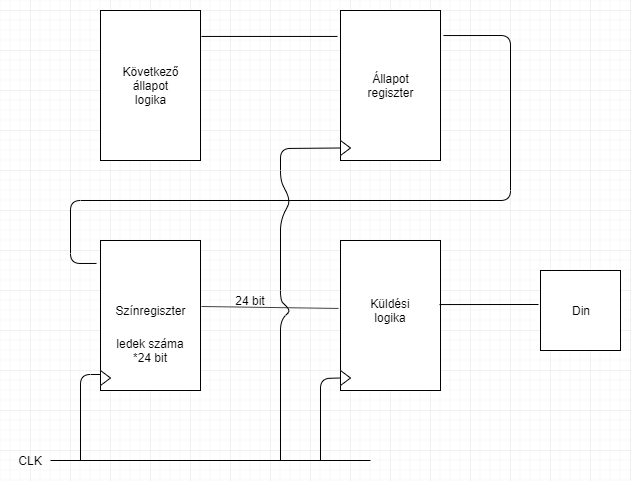
\includegraphics[scale=0.5]{tombvazlat.png}

\subsubsection{Küldési logika regiszter}

\noindent A küldési logika modul részletesebb lebontása: 

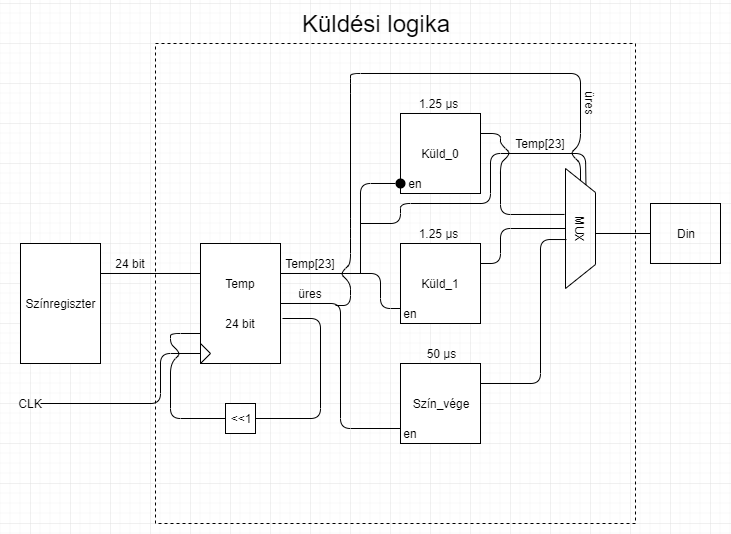
\includegraphics[scale=0.6]{kuldesi_logika.png}

\textbf{2019.10.28}

\indent Minden \textbf{led\_controll} modulhoz tartozik egy BRAM blokk és minden ilyen modul egy ledfűzért vezérel meg. Öt ilyen blokk megvezérel öt ledfűzért, ezáltal létrehozva a ledmátrixot.
Az órajel, start, reset, stop és data-rd jelek közösek minden modulnak.

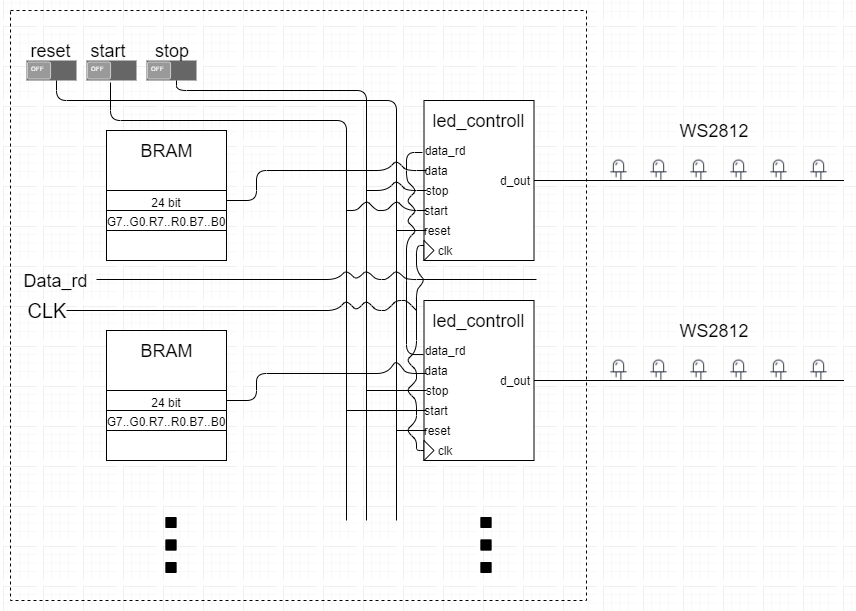
\includegraphics[scale=0.5]{tombvazlat2.png}